\documentclass[ignorenonframetext,]{beamer}
\setbeamertemplate{caption}[numbered]
\setbeamertemplate{caption label separator}{: }
\setbeamercolor{caption name}{fg=normal text.fg}
\beamertemplatenavigationsymbolsempty
\usepackage{lmodern}
\usepackage{amssymb,amsmath}
\usepackage{ifxetex,ifluatex}
\usepackage{fixltx2e} % provides \textsubscript
\ifnum 0\ifxetex 1\fi\ifluatex 1\fi=0 % if pdftex
  \usepackage[T1]{fontenc}
  \usepackage[utf8]{inputenc}
\else % if luatex or xelatex
  \ifxetex
    \usepackage{mathspec}
  \else
    \usepackage{fontspec}
  \fi
  \defaultfontfeatures{Ligatures=TeX,Scale=MatchLowercase}
\fi
% use upquote if available, for straight quotes in verbatim environments
\IfFileExists{upquote.sty}{\usepackage{upquote}}{}
% use microtype if available
\IfFileExists{microtype.sty}{%
\usepackage{microtype}
\UseMicrotypeSet[protrusion]{basicmath} % disable protrusion for tt fonts
}{}
\newif\ifbibliography
\hypersetup{
            pdftitle={Habits},
            pdfauthor={John Doe},
            pdfborder={0 0 0},
            breaklinks=true}
\urlstyle{same}  % don't use monospace font for urls

% Prevent slide breaks in the middle of a paragraph:
\widowpenalties 1 10000
\raggedbottom

\AtBeginPart{
  \let\insertpartnumber\relax
  \let\partname\relax
  \frame{\partpage}
}
\AtBeginSection{
  \ifbibliography
  \else
    \let\insertsectionnumber\relax
    \let\sectionname\relax
    \frame{\sectionpage}
  \fi
}
\AtBeginSubsection{
  \let\insertsubsectionnumber\relax
  \let\subsectionname\relax
  \frame{\subsectionpage}
}

\setlength{\parindent}{0pt}
\setlength{\parskip}{6pt plus 2pt minus 1pt}
\setlength{\emergencystretch}{3em}  % prevent overfull lines
\providecommand{\tightlist}{%
  \setlength{\itemsep}{0pt}\setlength{\parskip}{0pt}}
\setcounter{secnumdepth}{0}

\title{Habits}
\author{John Doe}
\date{March 22, 2005}

\begin{document}
\frame{\titlepage}

\begin{frame}{Overview}

\begin{figure}[!h]
  \centering
    
  \noindent 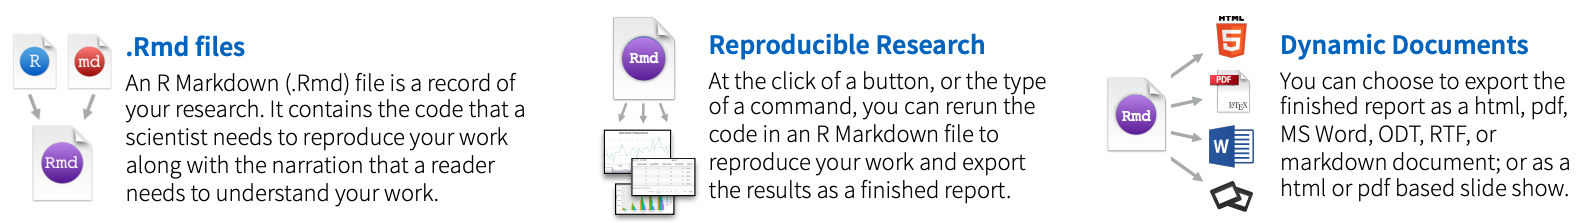
\includegraphics[width=\textwidth,height=\textheight,keepaspectratio]{/Users/KSauby/Documents/Projects/R-Markdown-Introduction/images/overview.png}
    
\end{figure}

\end{frame}

\begin{frame}{Breakfast}

\begin{figure}[!h]
  \centering
    
  \noindent 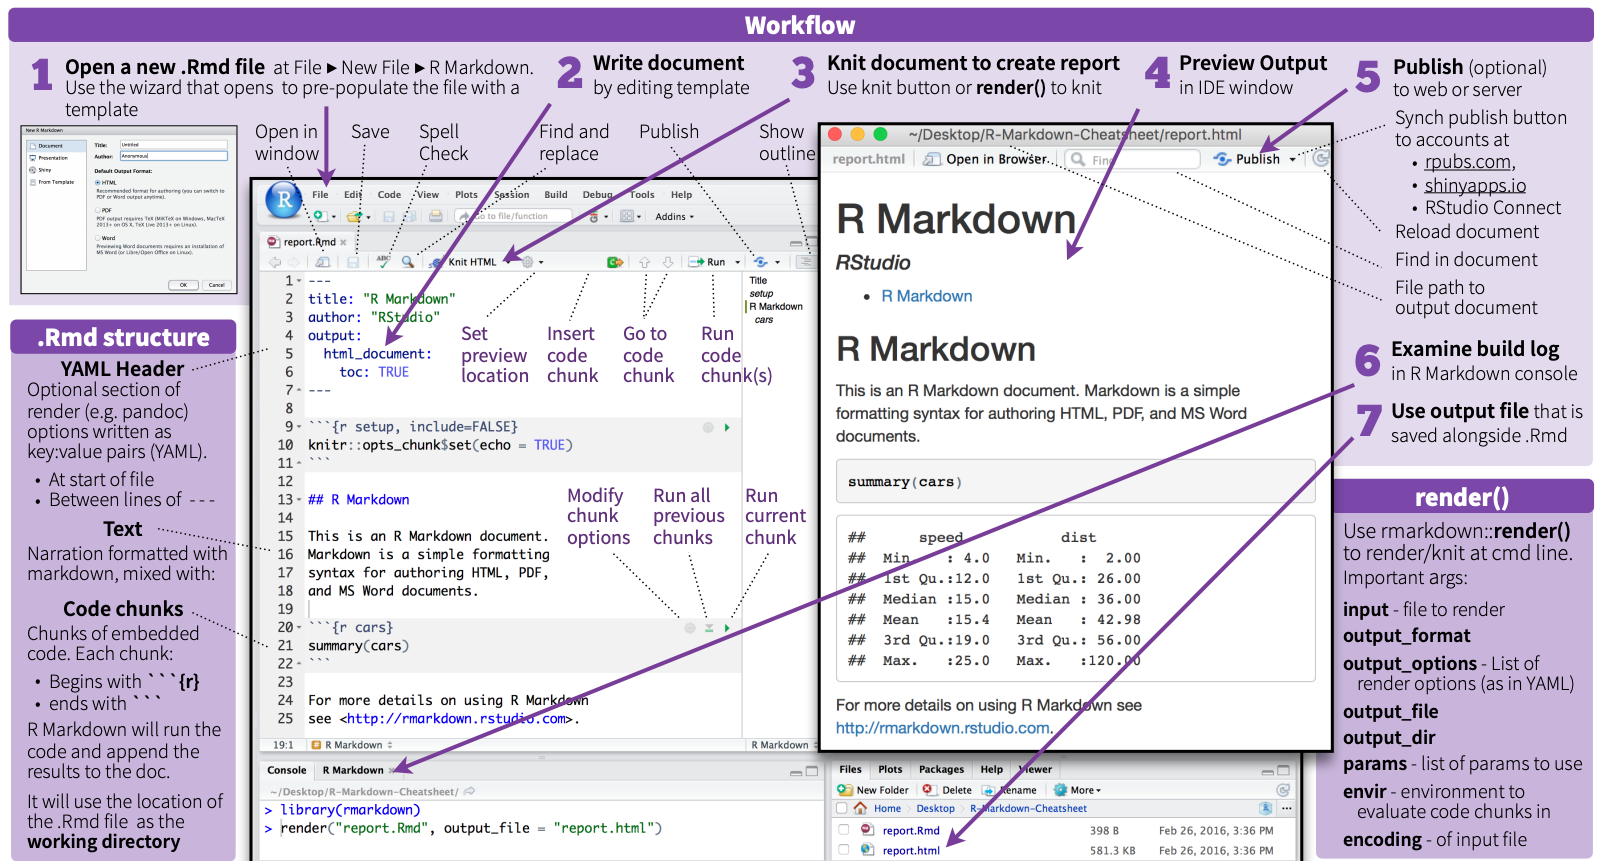
\includegraphics[width=\textwidth,height=\textheight,keepaspectratio]{/Users/KSauby/Documents/Projects/R-Markdown-Introduction/images/workflow.png}

\end{figure}

\end{frame}

\section{Citations + Google Scholar}\label{citations-google-scholar}

\begin{frame}{Set up Google Scholar, part 1}

Set up Google Scholar so that it shows your BibTex formatting for each
citation This assumes that you have a Google account

\end{frame}

\begin{frame}{Set up Google Scholar, part 2}

\end{frame}

\begin{frame}{Example - Addition Citations to your .bib}

\begin{itemize}
\tightlist
\item
  Now we can look up articles on Google Scholar and \emph{copy and
  paste} the BibTex citation to my ``bibliography.bib'' file
\item
  Rarely do I have to write the BibTex citation from scratch
\end{itemize}

\end{frame}

\begin{frame}{Why Use R Markdown for your Citations/Bibliography?}

\begin{itemize}
\tightlist
\item
  formats citations according to format of your choosing
\item
  compiles bibliography for you
\item
  when you re-compile your R Markdown document, the bibliography will be
  recreated as well -- ensures that bibliography is up-to-date -- no
  extras, no missing references
\end{itemize}

\end{frame}

\section{Other Benefits of Using R
Markdown}\label{other-benefits-of-using-r-markdown}

\begin{frame}{Tables}

\end{frame}

\begin{frame}{Tables and Figures}

\begin{itemize}
\tightlist
\item
  R Markdown numbers the tables and figures for you so you do not have
  to!
\end{itemize}

\end{frame}

\begin{frame}{R Markdown Vs. Microsoft Word}

Pros of R Markdown

\begin{itemize}
\tightlist
\item
  incorporate code directly into your document
\item
  you can hide text that you are ready to delete!
\end{itemize}

Cons of R Markdown

\begin{itemize}
\tightlist
\item
  track changes - not as easy to implement changes when you have to do
  it in R Markdown \#\# Bookdown Dissertation!
\end{itemize}

\url{https://github.com/ksauby/thesisdownufl}

\end{frame}

\begin{frame}{Resources}

\url{https://rmarkdown.rstudio.com/index.html}

\url{https://bookdown.org/yihui/rmarkdown/}

where to find csls

\end{frame}

\end{document}
